\documentclass[twocolumn]{aastex631}

% Packages
\usepackage{microtype}  % ALWAYS!
\usepackage{amsmath}
\usepackage{amsfonts}
\usepackage{amssymb}
\usepackage{multirow}

\definecolor{pink}{RGB}{232,132,161}
\definecolor{yellow}{RGB}{255,213,0}

\newcommand{\kc}[1]{\textcolor{yellow}{\textbf{kc: #1}} }
% \newcommand{\ecite}[1]{\textcolor{pink}{\textbf{: #1}} }
% \newcommand{\e}[1]{\textcolor{yellow}{\textbf{: #1}} }

\newcommand{\remove}[1]{\textcolor{red}{#1}}
\newcommand{\add}[1]{\textcolor{green}{#1}}

\newcommand{\mlg}{\ensuremath{M_{\rm LG}}}
\newcommand{\mmto}{\ensuremath{M_{\rm M31}}}
\newcommand{\mmw}{\ensuremath{M_{\rm MW}}}
\newcommand{\vtan}{\ensuremath{v_\textrm{tan}}}
\newcommand{\vrad}{\ensuremath{v_\textrm{rad}}}
\newcommand{\mud}{\ensuremath{\mu_\delta}}
\newcommand{\mua}{\ensuremath{\mu_\alpha^*}}
\newcommand{\bov}{\ensuremath{\boldsymbol{v}}}
\newcommand{\boldx}{\ensuremath{\boldsymbol{x}}}
\newcommand{\vtrav}{\ensuremath{\bov_{\rm travel}}}
\newcommand{\xtrav}{\ensuremath{\boldx_{\rm travel}}}
\newcommand{\pos}[2]{\ensuremath{\boldx_{\rm #1 \to #2}}}
\newcommand{\vel}[2]{\ensuremath{\bov_{\rm #1 \to #2}}}
\newcommand{\mwbary}{\ensuremath{\textrm{MW}_\textrm{bary}}}
\newcommand{\mwouter}{\ensuremath{\textrm{MW}_\textrm{halo}}}
\newcommand{\mwdisk}{\ensuremath{\textrm{MW}_\textrm{disk}}}
\newcommand{\reflabel}[1]{\ensuremath{^{\mbox{\scriptsize{#1}}}}}

% Style tweaks
% \renewcommand{\twocolumngrid}{\onecolumngrid}
% \setlength{\parindent}{1.1\baselineskip}
% \sloppy\sloppypar\raggedbottom\frenchspacing

%%%%%%%%%%%%%%%%%%%%%%%%%%%%%%%%%%%%%%%%%%%%%%%%%%%%%%%%%%%%%%%%%%%%%%%%%%%%%%%%
\shorttitle{Frequency of galaxy pairs}
\shortauthors{Chamberlain et al.}

%%%%%%%%%%%%%%%%%%%%%%%%%%%%%%%%%%%%%%%%%%%%%%%%%%%%%%%%%%%%%%%%%%%%%%%%%%%%%%%%
\graphicspath{{./}{../plots/pairs_plots/}}
% Missions
\newcommand{\project}[1]{\textsl{#1}}

% Packages / projects / programming
\newcommand{\package}[1]{\textsl{#1}}
\newcommand{\acronym}[1]{{\small{#1}}}
\newcommand{\github}{\package{GitHub}}
\newcommand{\python}{\package{Python}}
\newcommand{\astropy}{\package{Astropy}}

% Stats / probability
\newcommand{\given}{\,|\,}
\newcommand{\norm}{\mathcal{N}}
\newcommand{\pdf}{\textsl{pdf}}

% Maths
\newcommand{\dd}{\mathrm{d}}
\newcommand{\transpose}[1]{{#1}^{\mathsf{T}}}
\newcommand{\inverse}[1]{{#1}^{-1}}
\newcommand{\argmin}{\operatornamewithlimits{argmin}}
\newcommand{\mean}[1]{\left< #1 \right>}

% Non-scalar variables
\renewcommand{\vec}[1]{\ensuremath{\bs{#1}}}
\newcommand{\mat}[1]{\ensuremath{\mathbf{#1}}}

% Unit shortcuts
\newcommand{\Msun}{\ensuremath{\mathrm{M}_\odot}}
\newcommand{\Mjup}{\ensuremath{\mathrm{M}_{\mathrm{J}}}}
\newcommand{\kms}{\ensuremath{\mathrm{km}~\mathrm{s}^{-1}}}
\newcommand{\pc}{\ensuremath{\mathrm{pc}}}
\newcommand{\kpc}{\ensuremath{\mathrm{kpc}}}
\newcommand{\Mpc}{\ensuremath{\mathrm{Mpc}}}
\newcommand{\kmskpc}{\ensuremath{\mathrm{km}~\mathrm{s}^{-1}~\mathrm{kpc}^{-1}}}
\newcommand{\dayd}{\ensuremath{\mathrm{d}}}
\newcommand{\yr}{\ensuremath{\mathrm{yr}}}
\newcommand{\Myr}{\ensuremath{\mathrm{Myr}}}
\newcommand{\Gyr}{\ensuremath{\mathrm{Gyr}}}
\newcommand{\Kel}{\ensuremath{\mathrm{K}}}
\newcommand{\masyr}{\ensuremath{\mathrm{mas}~\mathrm{yr}^{-1}}}
\newcommand{\muasyr}{\ensuremath{\mu\mathrm{as}~\mathrm{yr}^{-1}}}

% Misc.
\newcommand{\bs}[1]{\boldsymbol{#1}}

% Astronomy
\newcommand{\DM}{{\rm DM}}
\newcommand{\feh}{\ensuremath{{[{\rm Fe}/{\rm H}]}}}
\newcommand{\df}{\acronym{DF}}

% TO DO
\newcommand{\todo}[1]{{\color{red} TODO: #1}}
\newcommand{\apw}[1]{{\color{blue} APW says: #1}}

% Projects
\newcommand{\gaia}{\textsl{Gaia}}
\newcommand{\gaiadr}{\textsl{Gaia}~\acronym{EDR3}}
\newcommand{\hst}{\textsl{HST}}
\newcommand{\ill}{\textsl{Illustris}}
\newcommand{\tng}{\textsl{IllustrisTNG}} 



% Affiliations
\newcommand{\affuofa}{University of Arizona, 933 N. Cherry Ave,
    Tucson, AZ 85721, USA}

%% This is the end of the preamble.  Indicate the beginning of the
%% manuscript itself with \begin{document}.

\begin{document}

\title{
  Frequency of galaxy pairs in the Illustris and IllustrisTNG cosmological simulations
}

\author[0000-0001-8765-8670]{Katie~Chamberlain}
\affiliation{\affuofa}

\author[0000-0003-0715-2173]{Gurtina Besla}
\affiliation{\affuofa}


\begin{abstract}
\end{abstract}

%%%%%%%%%%%%%%%%%%%%%%%%%%%%%%%%%%%
\section{Introduction} \label{sec:intro}


%%%%%%%%%%%%%%%%%%%%%%%%%%%%%%%%%%%
%%%%%%%%%%%%%%%%%%%%%%%%%%%%%%%%%%%
\section{Sample selection}\label{sec:methods}
Our sample data was obtained using a strict set of selection criteria, as outlined in this section.
In Sec.~\ref{sec:methods-sims}, we provide motivation for and details of the simulations utilized in this study.
Sec.~\ref{sec:methods-am} explains the abudance matching prescription used to associate stellar masses with the dark matter subhalos.
Sec.~\ref{sec:methods-crit} provides a detailed outline of our selection criteria and process for picking pairs.
Finally, Sec.~\ref{sec:methods-counts} gives an overview of the properties of our sample.

%%%%%%%%%%%
%%%%%%%%%%%
\subsection{Simulation details}\label{sec:methods-sims}
% what is it that we are trying to study? why use illustris?
To understand the occurance rate and separations of typical galaxy pairs in a cosmological context, we require a simulation that provides a large statistical sample of pairs in both the dwarf and massive galaxy regime. 
Thus, we are limited in our simulation choice to large-volume cosmological simulations. 
However, we also require high resolution simulations such that the dwarf subhalos are resolved well enough to ensure robust statistics at the low mass end, and so we are not limited by our inability to resolve objects down to halo masses of $M_{\rm halo}\approx1\times 10^9\, \Msun$.

% Baryonic processes
Baryonic process are known to affect the dark matter halo structure of low mass ($M_*<1\times10^9\Msun$) subhalos in simulations~\citep[see e.g.][and references therein]{Sales:2022}.
Additionally, the shallow potential well of dwarf galaxies compared to their massive counterparts may lend themselves more easily to disruption from baryonic processes such as supernova feedback, which could change the occurance rate of low mass subhalos in hydrodynamic simulations \kc{check and see if they looked at this in the TNG100 galaxy paper}.
To study the effect of baryonic processes on the rate and separation of pairs, we require cosmological simulations which have both dark matter only runs and to full hydrodynamics.

% details of Illustris and Illustris TNG
The \textit{Illustris Project} ~\citep{vogelsberger14A,nelson15} and \textit{IllustrisTNG Project}~\citep{TNG1, TNG2, TNG3, TNG4, TNG5} are a set of N-body and hydrodynamic cosmological simulations which are perfectly suited for such a study. 
We use the dark matter only and full hydrodynamic runs of both the \ill-1 and \tng100-1 simulations to explore the connection between pairs and baryonic processes. 
Each of these simulations follows the dynamical evolution of $1820^3$ dark matter particles from $z=127$ to $z=0$ through a periodic volume of roughly $100^3$ Mpc$^3$. 
The \ill{} simulations follow a cosmology consistent with \textit{WMAP-9}~\citep{hinshaw13}, while the \tng{} simulations are consistent with \textit{Planck2015}~\citep{Planck2015}.
Specifically, we use the \textit{Illustris-1-Dark}, \textit{Illustris-1}, \textit{TNG100-1-Dark}, and \textit{TNG100-1} simulations (hereafter \illd, \illh, \tngd, and \tngh{} respectively, see Table~\ref{table:sim} for details).

% deets on the hydrodynamics of 
\kc{hydrodynamics details on the difference between the two hydro simulations. also include differences between the two dark simulations, if there are any besides the cosmology. }

% subfind, sublink, and groups and subhalos
We utilize the group catalogs produced by the \texttt{SUBFIND} algorithm ~\citep{springel01,dolag09}. 
These catalogs consist of halos (or "groups"), defined using the Friends-of-Friends (FoF) algorithm~\citep{davis85} to link nearby particles, and their associated subhalos, which are over-dense and gravitationally bound dark matter structures.
We also use the merger trees provided by the \texttt{SUBLINK} algorithm \citep{gomez15}, which tracks subhalos between snapshots using their particle data, in order to trace the mass growth and merger histories of our subhalos.


\begin{table*}[htb]
\begin{tabular}{l|llll}
 & \illd & \illh & \tngd & \tngh\\\hline\hline
 L$_{\rm Box}$ [Mpc] & 106.5 & 106.5 & 110.7 & 110.7 \\
m$_{\rm DM}$ [M$_\odot$] & 7.5$\times10^6$ & 6.3$\times10^6$ & 8.9$\times10^6$ & $7.5\times10^6$\\
m$_{\rm gas}$ & -- & $1.3\times 10^{6}$ & -- & $1.4\times 10^{6}$ \\\hline
\end{tabular}
\caption{\label{table:sim}Parameters of the Illustris simulations used in this analysis.}
\end{table*}



%%%%%%%%%%%
%%%%%%%%%%%
\subsection{Abundance matching prescription}\label{sec:methods-am}
% Why do we need stellar masses?
One of the goals of this study is to determine the impact of baryonic physics on the occurance rate and typical separations of galaxy \kc{subhalo?} pairs in cosmological simulations. 
However, selecting halo pairs by stellar mass ratio using the stellar masses provided by the simulations is not possible in the dark matter only runs. 
Thus, in order ensure the dark matter only and full hydrodynamic samples are self-consistent, we need to associate each of the selected subhalos with a realistic stellar mass.

% What is abundance matching
Abundance matching is one such method of associating a dark matter halo with a stellar mass, assuming a galaxy would form in a halo of that mass. 

However, there is large scatter in the stellar-mass-halo-mass (SMHM) relationship, especially in the dwarf halo regime. 



% How do we utilize it? 
In particular, we use the abundance matching relationship presented in~\citet{moster13}, which provides an analytic recipe to paint stellar masses onto dark matter halos. 
The~\citet{moster13} relationship is a redshift-evolving function of the halo mass, and includes terms to account for the systematic scatter in the SMHM relationship, with larger scatter at lower halo masses.
\kc{why moster instead of another AM relationship? most closely represent data at lower mass? }

To assign stellar masses to each of the dark matter halos, we assume that the stellar mass of both the primary and secondary halo can change as a function of redshift after the secondary has entered the primary's halo and do not immediately cease star formation.
This assumption is consistent with findings from~\cite{Akins2021}, which found that massive dwarf satellites ($M_*\approx 10^8-10^9\, \Msun$) entering MW-mass host halos are rarely quenched, and with~\cite{geha13} which finds that isolated dwarfs ($>1\Mpc$ from a MW-type galaxy) are often star forming and rarely quenched.
Additionally,~\citet{Munshi2021} found that the stellar mass of subhalos at $z=0$ in the XX simulations are more closely correlated with the peak halo mass than the $z=0$ halo mass for halos with peak halo mass $10^8<M_{\rm peak}<10^{11} \Msun$. 

Thus, we treat each of the subhalos as centrals according to the~\citet{moster13} prescription, using the current snapshot redshift and the peak halo mass of the subhalo to calculate the stellar mass. 
This additionally allows us remain robust to scenarios in which a secondary may have formed most of its stars, and then lost a significant portion of its dark matter content through tidal interactions with a primary, but will retain the bulk of its stellar content.

We create 1000 stellar mass realizations from the SMHM relationship, thus accounting for the systematic uncerntainy in subhalo stellar masses, which will allow us to average our results over all 1000 realizations 

%%%%%%%%%%%
%%%%%%%%%%%
\subsection{Selection criteria}\label{sec:methods-crit}
\begin{enumerate}
  \item Select groups in some group range that encompasses MCs and MW-M31
  \item For every subhalo in every group with halo mass >1e9Msun, use merger trees to get the maximum masses.
  \item Generate 1000 stellar mass realization using abundance matching so we can account for the spread in the relationship
  \item Generate catalog at each redshift containing: 
  \begin{itemize}
    \item For each realization, and in each group with a single subhalo, add the subhalo and it's properties to a catalog of single halos.
    \item For each realization, and in each group with 2+ halos, find most massive halo by stellar mass, and the second most massive halo by stellar mass, then add to pair catalog. 
    \item If a group has 3+ halos, check the stellar mass of the third most massive object, and see if it is a major/minor companion of the secondary. If not, teritary flag = 0. Otherwise =1.
  \end{itemize}
  \item Select dwarf primaries: for full catalog, most massive halo (in "pairs") or single halos with stellar mass $1\times10^{8} < \msam < 5\times10^{9} \Msun$. 
  \item Select dwarf pairs: for full pair catalog, any pair with stellar mass ratio between 1-1/4 (major pairs) or between 1/4-1/10 (minor pairs). All pairs is the union of these two sets. Any pair or single halo that is outside of these two sets is an "unpaired" halo. Note that unpaired can still have very minor companions. 
\end{enumerate}

The lower mass threshold for subhalos that constitute our dwarf pairs have a halo mass greater than $1\times10^9\Msun$, such that each of our halos are resolved into at least 100 particles in each simulation.  
\kc{why 100?} 

\subsection{Counts and distributions}\label{sec:methods-counts}

\begin{itemize}
  \item Introduce simulations
  \item outline selection steps
  \item dwarf pairs
  \item massive pairs
  \item include table with parameters used for pairs
  \item plots
    \begin{itemize}
      \item distribution plots
      \item counts plots
    \end{itemize}
\end{itemize}


% selection criterion
\begin{table*}[htb]
  \centering
    \begin{tabular}{lcc}
     & Dwarf Pairs & Massive Pairs \\\hline\hline
    % Group Mass & $8\times10^{10} < \rm M_g < 5\times10^{11} M_\odot$ & $1\times10^{12} < \rm M_g < 4\times10^{12} M_\odot$  \\
    % Subhalo Max Mass &  &  \\
    % Subhalo Current Mass & $>1\times10^{10} \Msun$ & $> 5\times10^{11} \Msun$ \\
    Primary &$1\times10^{8} < \msam < 5\times10^{9} \Msun$ & $5\times10^{9} < \msam < 1\times10^{11} \Msun$\\\hline
    \end{tabular}
    \caption{\label{table:mass}Selection criteria for dwarf and massive pairs.}
    \end{table*}

% equivalent snapshot table
\begin{table*}[]
  \centering
  \begin{tabular}{l|cc|cccc} % increase this to 7 columns
    \hline \hline
   & \multicolumn{2}{c|}{Snapshot number} & \multicolumn{4}{c}{Number of primaries}\\
   & \ill & \tng  & \illd & \illh & \tngd & \tngh \\ 
  \hline
  z = 0   &   135  &   99   &&&&\\
  z = 1   &   85   &   50   &&&&\\
  z = 2   &   68   &   33   &&&&\\
  z = 3   &   60   &   25   &&&&\\
  % z = 3.7   &   54   &   21   \\
  \hline \hline
  \end{tabular}
  \caption{\label{tab:equiv-snapshot} The snapshot number of the original \ill\ and the \tng\ simulations at redshifts $z=0-3$, as well as the number of total dwarf (massive) primaries that were selected with $1\times 10^{8} < \msam < 5\times 10^{9} \rm M_\odot$ ($5\times 10^{9} < \msam < 1\times 10^{11} \rm M_\odot$) in XX abundance matching realizations. \kc{fill in with numbers after doing more realizations} \kc{include takeaway}}
  \end{table*}



%%%%%%%%%%%%%%%%%%%
%% dwarf figures %%
%%%%%%%%%%%%%%%%%%%
\begin{figure*}[htb]
  \centering
  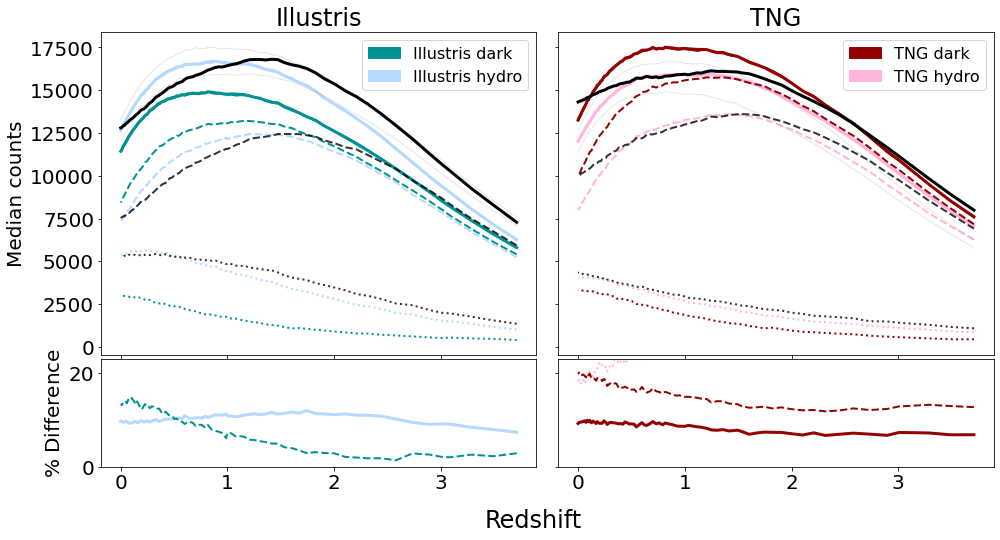
\includegraphics[width=\textwidth]{counts_dwarfs.png}
  \caption{Median counts of dwarf primaries in \ill{} and \tng{} \kc{add "dwarf" somewhere to plot}. The number of dwarf primaries peaks at $z~0.75$. TNG has higher halo count than Illustris. However, the difference between the number of halos in both dark simulations is substantial. Additionally, in Illustris, hydro halos outnumber dark halos. In TNG, the opposite is true, where dark halos outnumber hydro halos. In Illustris, this can be accounted for by the discrepant number of unpaired halos (dotted), while in TNG, the difference is dominated by pairs. 
    }
  \label{fig:counts-dwarfs}
\end{figure*}

\begin{figure*}[htb]
  \centering
  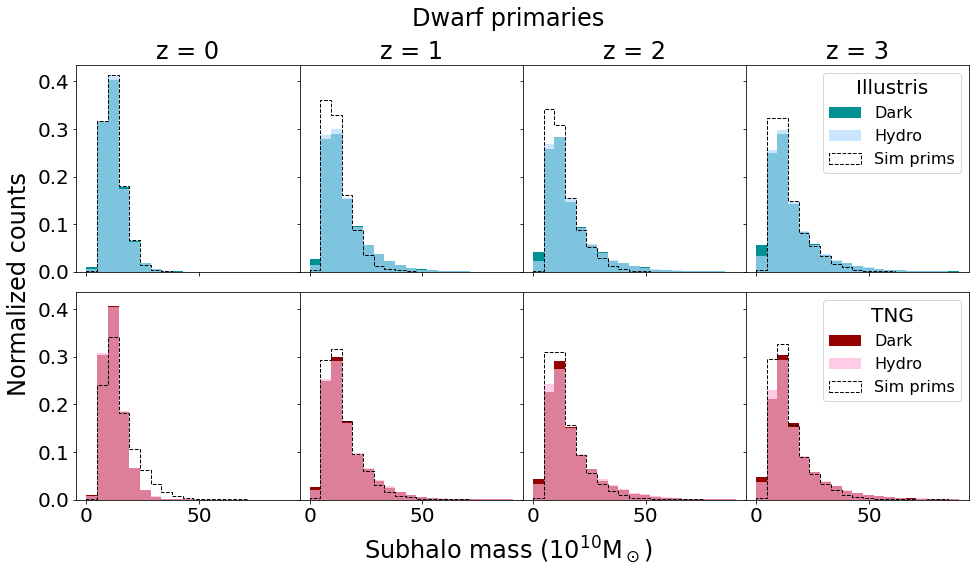
\includegraphics[width=\textwidth]{distributions_mass_dwarf.png}
  \caption{Normalized distribution of the subhalo mass of dwarf primaries at four different redshifts. The subhalos in the dark and hydro simulations for both \ill{} (turquoise and light blue) and \tng{} (red and light pink) were chosen such that the stellar mass from the abundance matching prescription is $1\times 10^{8} < \msam < 5\times 10^{9} \rm M_\odot$. The black dashed lines represent the distribution of halos chosen by \mssim.
  The mass distributions for \illd{} and \illh{} are nearly identical at all redshifts, however, while the mass distribution for halos chosen by their simulation stellar mass closely match the \ill{} distribution at $z=0$, the \mssim{} distribution skews towards lower subhalo masses than the \msam{} distributions at $z=1,2,3$. Similarly, the \tngd{} and \tngh{} distrbutions are consistent at all redshifts, however the population of subhalos chosen by simulation stellar mass have higher masses at $z=0$ and lower masses at $z=1,2,3$ than the \msam{} distributions. 
  The approximate equivalence of the dark and hydro distributions in both simulations confirm that we are investigating a similar population of halos between the dark and hydro runs of each simulation. Additionally, the distributions for \ill{} and \tng{} follow the same evolution over time, so the population of subhalos we are considering is consistent between simulations. 
    }
  \label{fig:dist-mass-dwarf}
\end{figure*}

\begin{figure*}[htb]
  \centering
  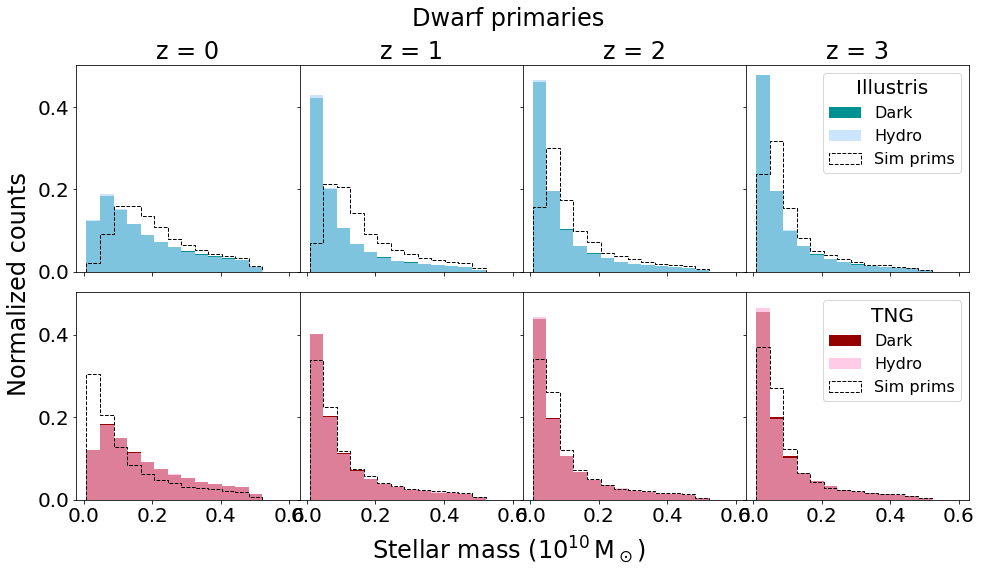
\includegraphics[width=\textwidth]{distributions_stellarmass_dwarf.png}
  \caption{Normalized distribution of the stellar mass from abundance matching of dwarf primaries at four different redshifts. The subhalos in the dark and hydro simulations for both \ill{} (turquoise and light blue) and \tng{} (red and light pink) were chosen such that the stellar mass from the abundance matching prescription is $1\times 10^{8} < \msam < 5\times 10^{9} \rm M_\odot$. 
  The black solid lines represent the simulation values of the stellar mass for the same population of halos chosen by their abundance matching stellar mass. 
  The black dashed lines represent the distribution of halos chosen by their simulation stellar mass, $1\times 10^{8} < \mssim < 5\times 10^{9} \rm M_\odot$.
  The mass distributions for \illd{} and \illh{}, as well as \tngd{} and \tngh{}, are nearly identical at all redshifts. 
  However, the distributions chosen by the simulation stellar mass differ drastically between the two simulations. At $z=0$, there are many more low \mssim{} halos in \tng{} than in \ill{}. In addition, the simulation stellar masses in the \ill{} simulation tend to be more massive than those from abundance matching at all redshifts. 
  The abundance matching stellar mass and simulation stellar mass distributions in \tng{} are similar at $z=1,2,3$, with more low stellar mass halos in the abundance matching case, while at $z=0$, the simulation stellar masses are significantly lower than the distribution from abundance matching. 
  \kc{what does this mean?? } 
    }
    \label{fig:dist-stellmass-dwarf}
  
\end{figure*}


%%%%%%%%%%%%%%%%%%%%%
%% massive figures %%
%%%%%%%%%%%%%%%%%%%%%
\begin{figure*}[htb]
  \centering
  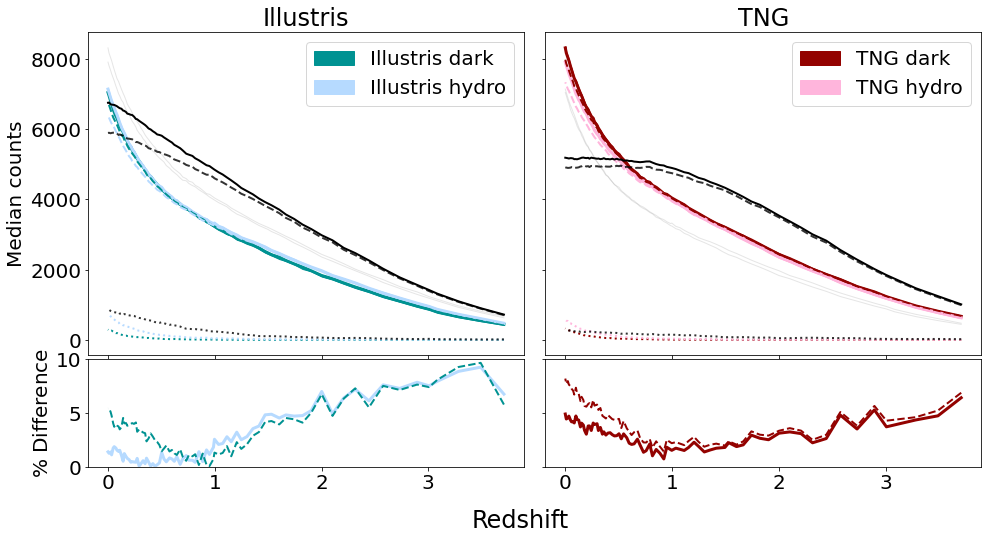
\includegraphics[width=\textwidth]{counts_massive.png}
  \caption{No turn over, instead, monotonically increasing towards a peak at low z. No significant fraction of halos that are lone subhalos. The largest differences between the hydro and dark simulations in both cases are at low z, where the counts start to diverge. TNG has a higher number of massive halos primaries than Illustris. The difference between dark and hydro is large in TNG, and at low z, the main driver of this difference is in the pairs, as opposed to the lone halos. This is not the case in Illustris, where both the pairs and unpaired halos contribute equally to the difference between dark and hydro, in opposite way! Weird… \kc{add "massive" somewhere to plot}
    }
  \label{fig:counts-massive}
\end{figure*}

\begin{figure*}[htb]
  \centering
  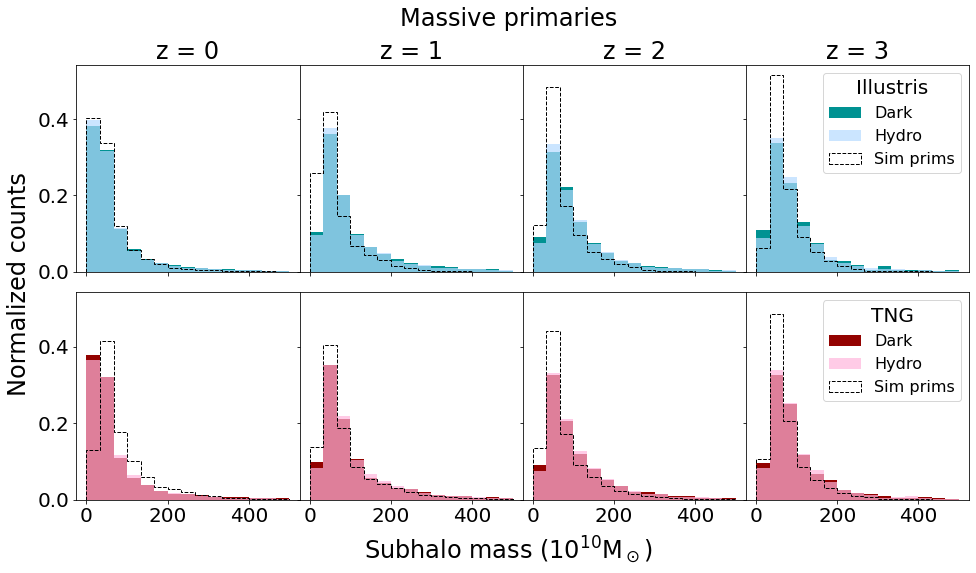
\includegraphics[width=\textwidth]{distributions_mass_massive.png}
  \caption{There is little variation between dark and hydro, and Illustris and TNG. Like the dwarf primaries, the distribution of selected primaries by simulation mass at z=0 in Illustris nearly overlays the distribution from the am mass. In addition, the z=0 sim mass selection in TNG is a higher mass distribution than those selected by am mass. It appears that the mass distributions in both Illustris and TNG change significantly between z=3 and z=0, but the sim selected list in TNG does not change. However, for both simulation, at z=1,2,3, the am mass selected primaries have, on average, higher mass than the sim mass selected primaries. \kc{add takeaway} 
    }
  \label{fig:dist-mass-massive}
\end{figure*}

\begin{figure*}[htb]
  \centering
  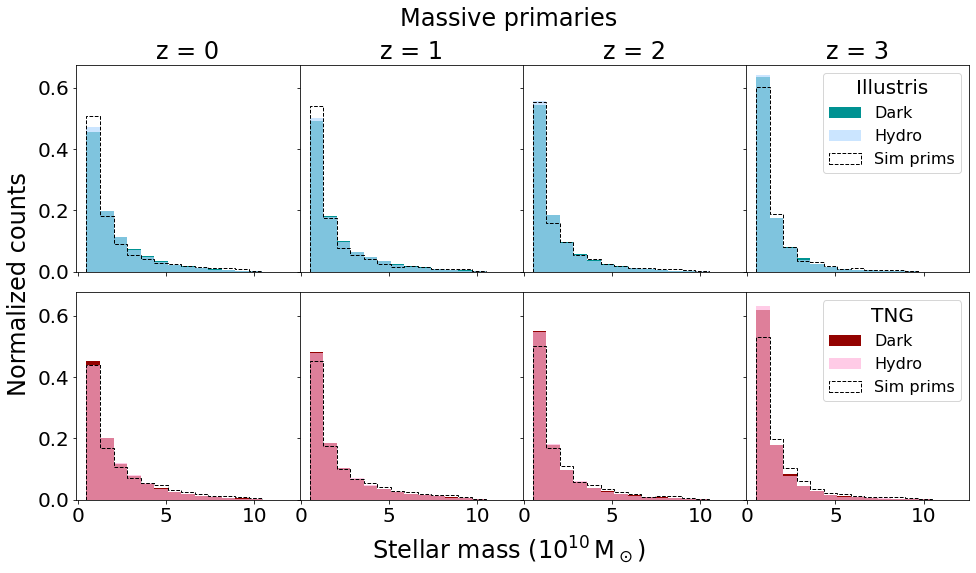
\includegraphics[width=\textwidth]{distributions_stellarmass_massive.png}
  \caption{The dark and hydro distributions, as well as the Illustris and TNG distributions, are all similar. There is also good agreement with the stellar mass of halos selected with the simulation stellar mass (this tells me that the AM relationship better matches what we see in sims at high mass but not at low mass). The black solid line does not match well, but I'll be removing it anyways. \kc{ add takeaway message}
    }
  \label{fig:dist-stellmass-massive}
\end{figure*}

%%%%%%%%%%%%%%%%%%%%%%%%%%%%%%%%%%%

\section{Results}
\label{sec:results}


%%%%%%%%%%%%%%%%%%%%%%%%%%%%%%%%%%%
\section{Discussion}
\label{sec:discussion}


%%%%%%%%%%%%%%%%%%%%%%%%%%%%%%%%%%%
\section{Summary and Conclusions}
\label{sec:summary}

%%%%%%%%%%%%%%%%%%%%%%%%
%%%%%%%%%%%%%%%%%%%%%%%%

\bibliography{refs}{}
\bibliographystyle{aasjournal}

\end{document}
